\begin{figure}[htb!]
\centering
\begin{tabular}{ccc}
%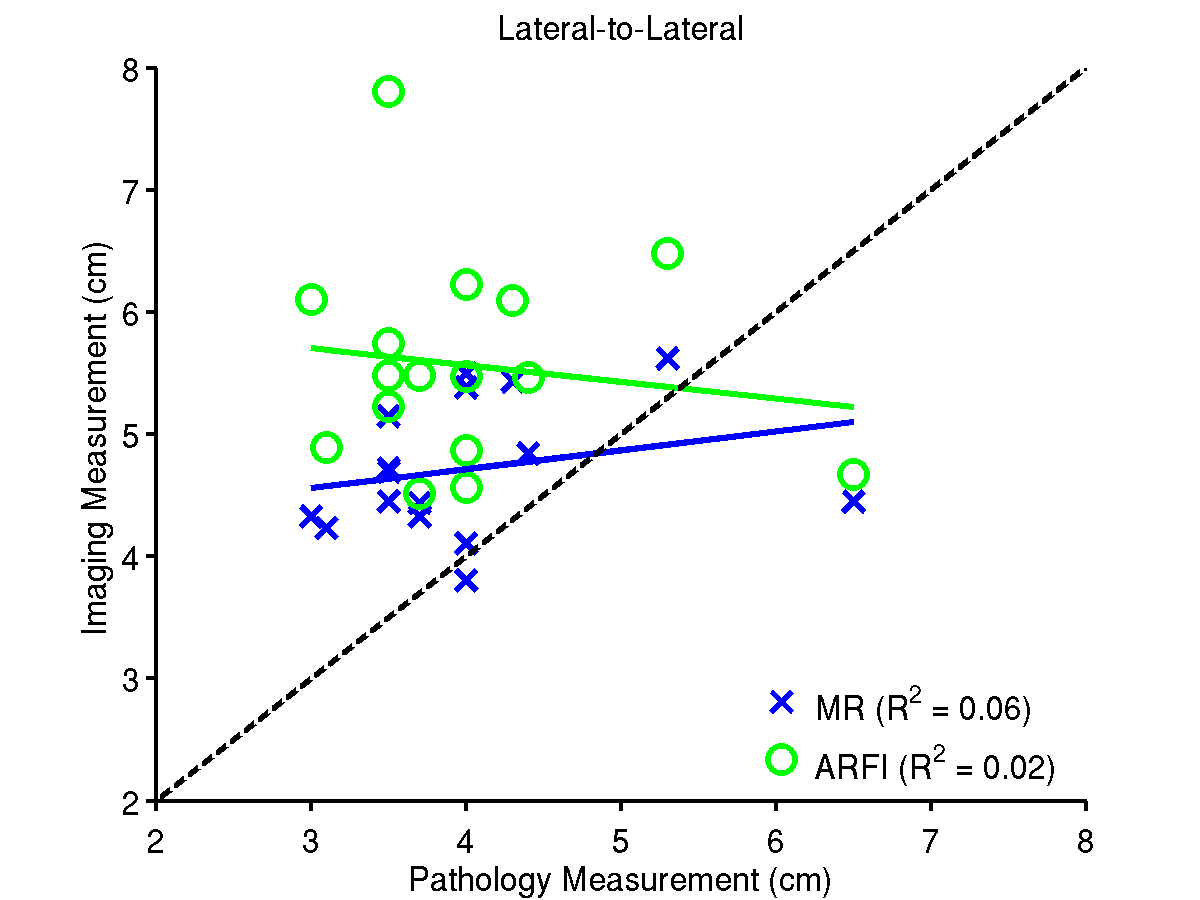
\includegraphics[width=0.3\linewidth]{figs/Lateral-to-Lateral} &
%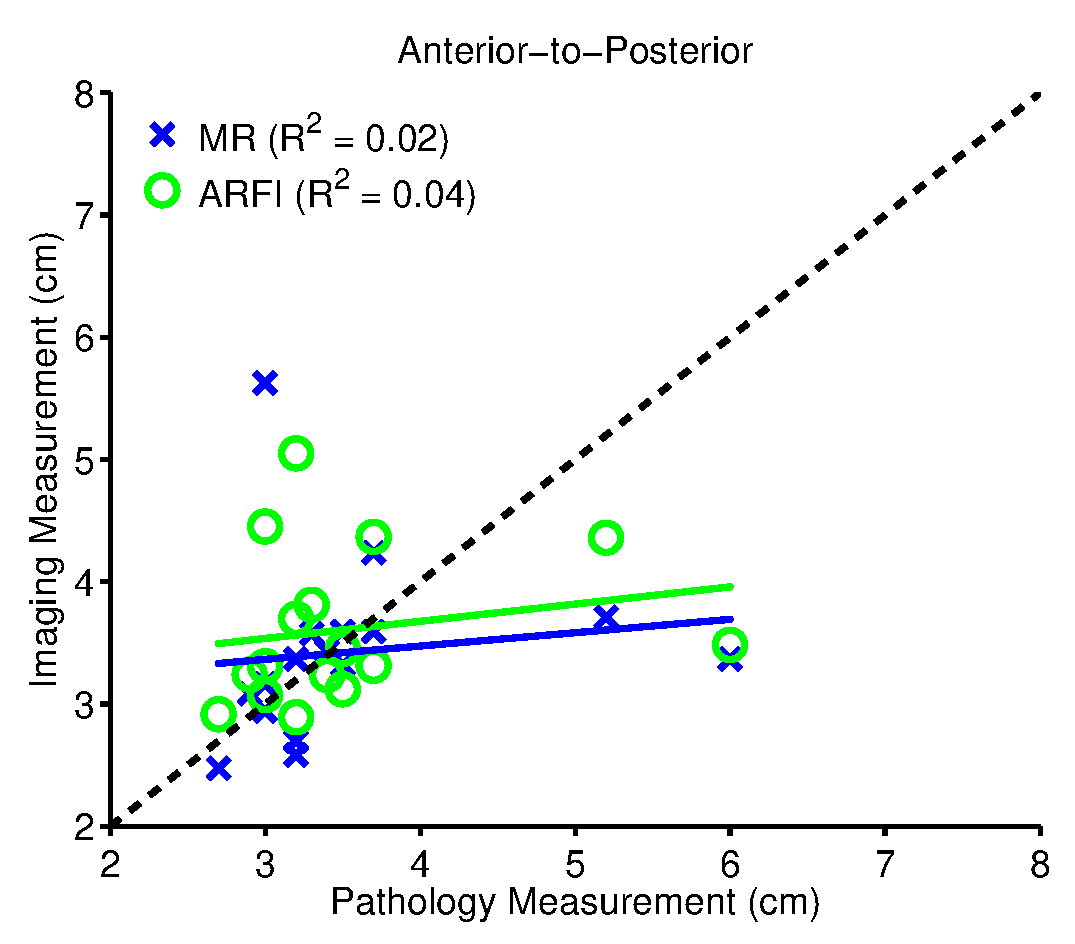
\includegraphics[width=0.3\linewidth]{figs/Anterior-to-Posterior} &
%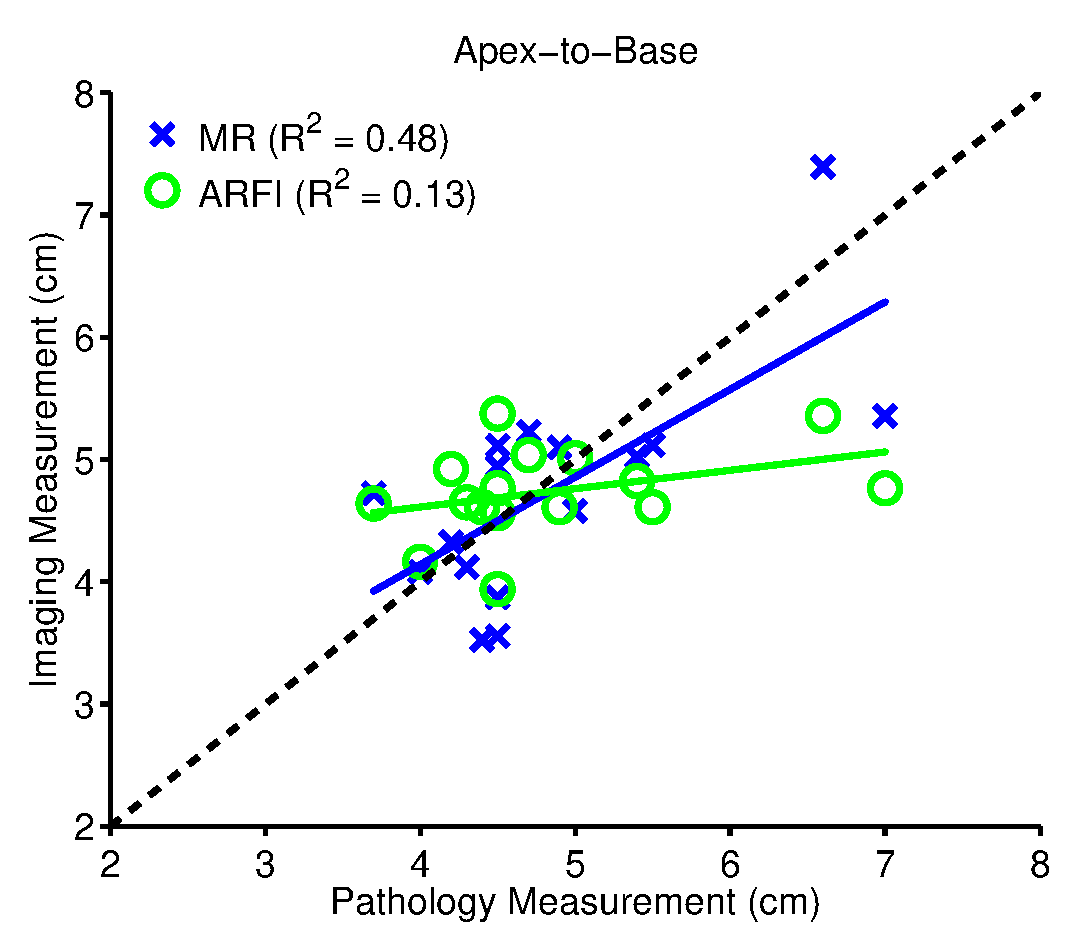
\includegraphics[width=0.3\linewidth]{figs/Apex-to-Base} \\
%(a) & (b) & (c) \\
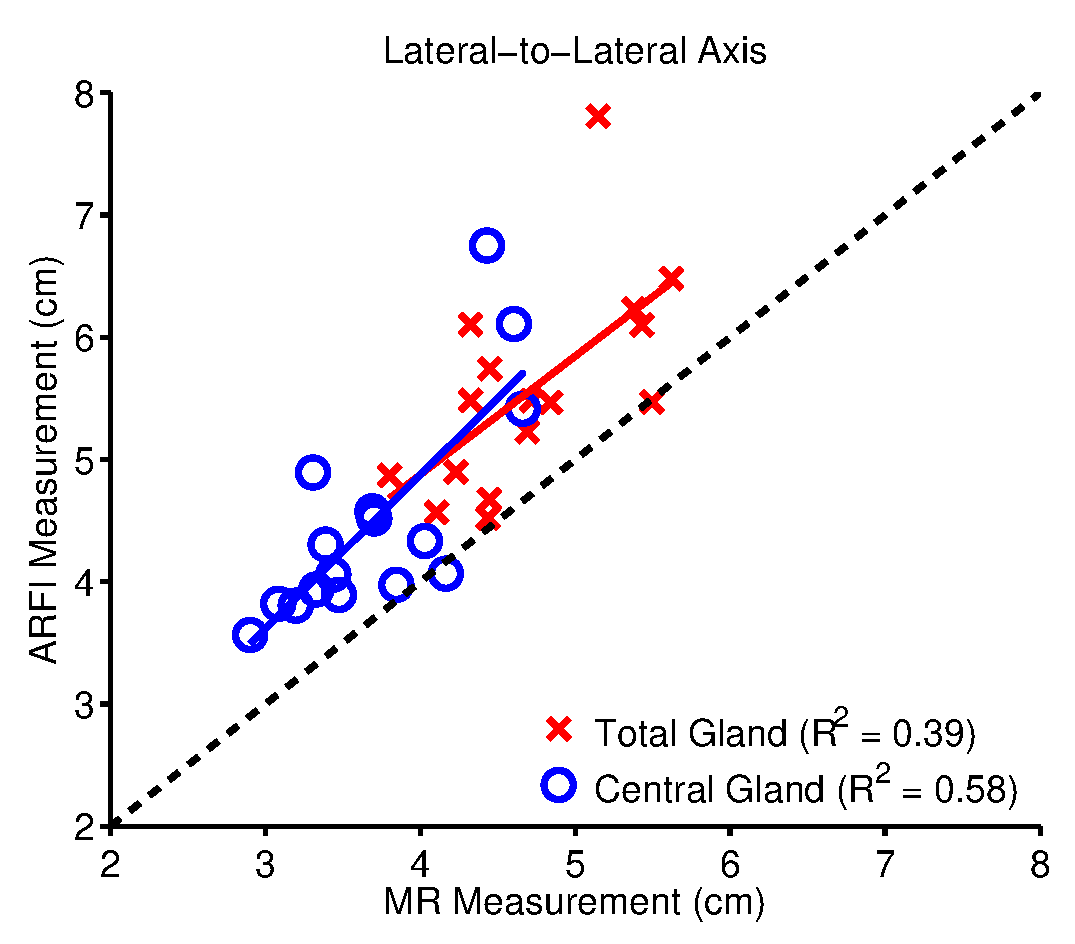
\includegraphics[width=0.3\linewidth]{figs/Imaging_Lateral-to-Lateral} &
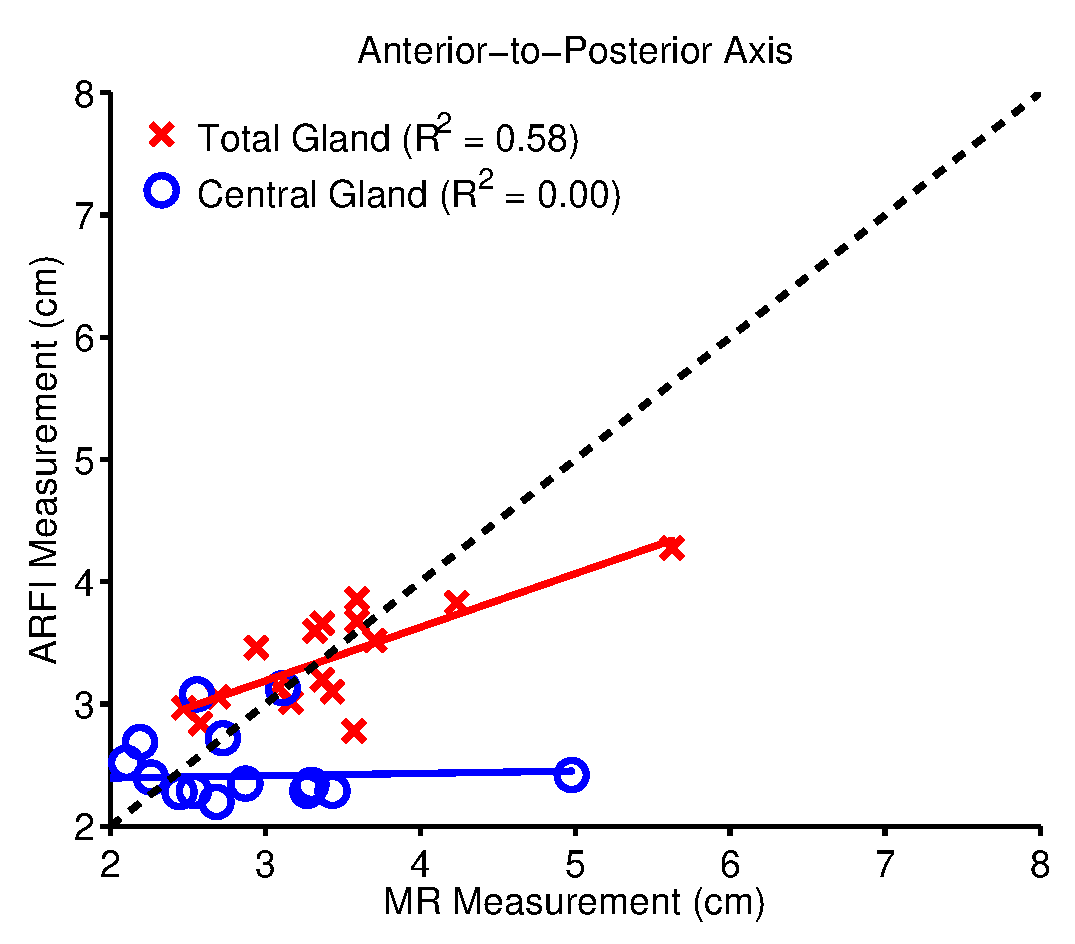
\includegraphics[width=0.3\linewidth]{figs/Imaging_Anterior-to-Posterior} &
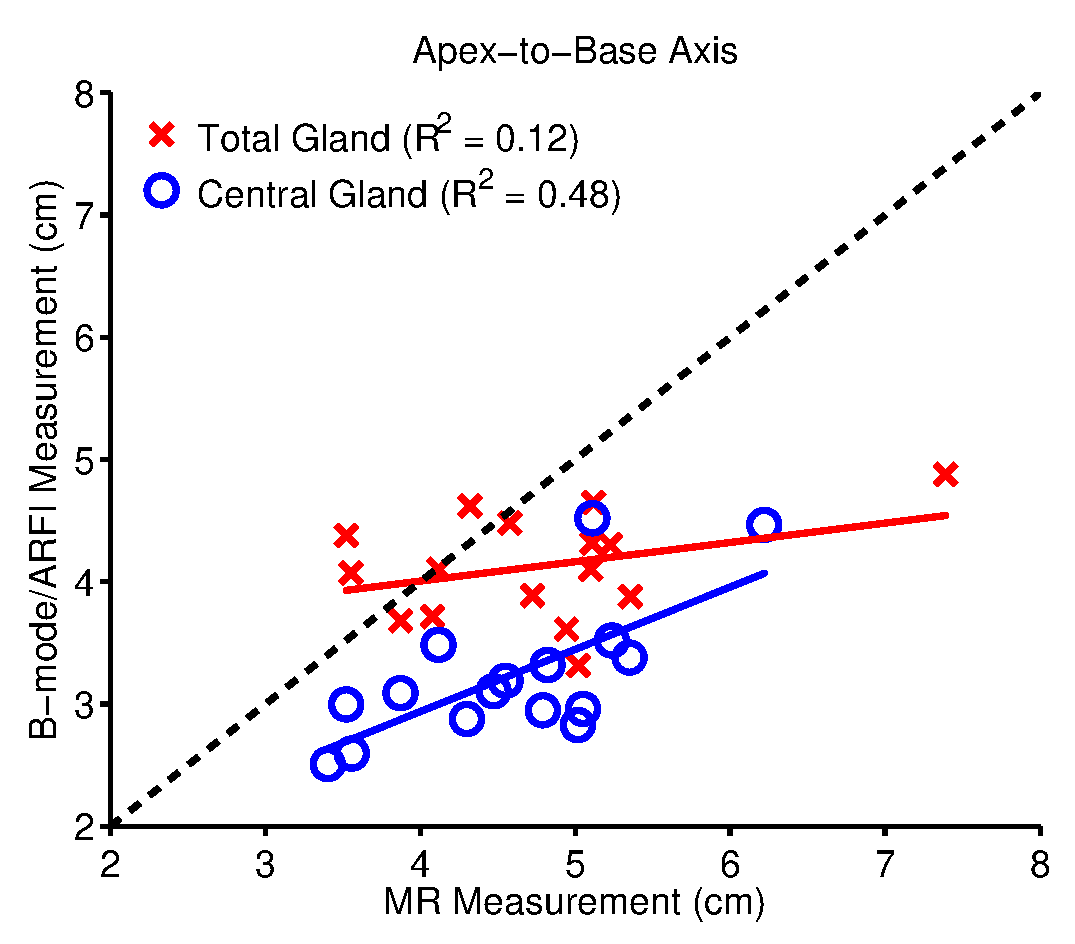
\includegraphics[width=0.3\linewidth]{figs/Imaging_Apex-to-Base} \\
(a) & (b) & (c) \\
%(d) & (e) & (f) \\
\end{tabular}
\caption{Measurements of the prostate dimensions along the three standard
    anatomic axes: lateral-to-lateral (a), anterior-to-posterior (b) and
    apex-to-base (c).  The correlation between the MR and ARFI imaging axis
    measurements was performed in each orientation for the total gland (black
    crosses) and central gland (red circles).  The black dashed-line represents
    the projection of perfectly-correlated measurements between imaging and
    patholoy.  The over-/under-estimation of each imaging modality relative to
    gross pathology and each other is summarized in
    Table~\ref{tab:mr_arfi_axes_error}.} 
\label{fig:mr_arfi_path_axes}
\end{figure}
